\singlespacing
\chapter{Microespectrómetro}
\label{chap:microsp}
\spacing{1.5}

\hspace{0.5cm}En el Capítulo \ref{chap:zeiss} se realizó una descripción cuantitativa de los defectos: se determinó su área, su diámetro equivalente, la cantidad de defectos presentes en cada banda, etc. Dicho análisis permitió entender las especificaciones técnicas de \textit{scratch \& dig} y de la ISO 10110, lo que resulta fundamental para establecer las bases de futuros acuerdos con los fabricantes de los componentes ópticos. Al mismo tiempo, los resultados de la población de defectos en general [\ref{sec:defpob}] detectados con el algoritmo permitieron establecer los criterios de diseño óptico del microespectrómetro que se explica en el presente capítulo.

Como se explicó en el Capítulo \ref{chap:introd}, un microespectrómetro es un instrumento de medición híbrido que integra la capacidad de magnificación y de resolución ópticas de un microscopio con la capacidad de inferir las propiedades ópticas de un material de un espectrómetro. En este capítulo se describe la construcción y montaje de un microespectrómetro que permitió realizar una caracterización de las propiedades ópticas del filtro y de sus defectos a través de los espectros de transmisión [\ref{sec:montcontmsp}]. En la Sección \ref{sec:prot0} muestran las características del primer prototipo desarrollado con equipamiento disponible en el laboratorio. Dicho prototipo en conjunto con los resultados y análisis del Capítulo \ref{chap:zeiss} permitieron establecer los criterios de elección de la fuente de luz y del espectrómetro [\ref{sec:fteluzyesp}], determinar la longitud del recorrido y la precisión mínima necesaria de la platina que se desarrolló [\ref{sec:platina}] y la resolución óptica necesaria del microscopio desarrollado para caracterizar los defectos de diámetro mayores a 20$\mu m$ de diámetro [\ref{sec:disop}]. Luego se explica el proceso de montaje y alineación preliminar del microespectrómetro [\ref{sec:montalin}] así como su puesta en foco y la determinación de la resolución espacial [\ref{sec:focoresol}]. Posteriormente se explica la integración de una cámara web al microespectrómetro lo que permitió la adquisición simultánea de imágenes digitales y de espectros de transmisión y cuya área de adquisición fue elegida con un \textit{joystick} y visualizada en vivo a través de una interfaz gráfica [\ref{sec:camwebgui}].

Asimismo, se muestran los resultados de los espectros de transmisión de cada banda del filtro y su comparación con la hoja de datos reportada por el fabricante [\ref{sec:espectransm}]. Finalmente, se muestran los resultados de la caracterización espectral de los defectos denominados manchas ó defectos de transmisión [\ref{sec:defctma}] y de los agujeros ó huecos [\ref{sec:defctag}].

\singlespacing
\section{Prototipo 0 \href{https://github.com/jrr1984/thorlabs_step_motors_ZST213B/tree/master/barrido/std}{\faGithub}}
\label{sec:prot0}
\spacing{1.5}

\hspace{0.5cm}El desarrollo del prototipo 0 que se muestra en esta sección permitió por un lado establecer los criterios de elección de la fuente de luz y del recorrido y la precisión necesarias de la platina desarrollada para poder adquirir el espectro e imágenes del filtro completo. Como buena práctica de prototipado de instrumentos de medición se utilizaron componentes y equipamiento disponibles en el laboratorio, es decir que no se incurrió en gastos adicionales de dinero a excepción del costo del material de las impresiones 3D del soporte del filtro. Por otro lado, a partir del desarrollo del software automatizado de adquisición y de visualización de los resultados de este prototipo se establecieron las características deseadas y esperadas del prototipo final desarrollado. De esta manera, el prototipo permitió establecer la factibilidad del desarrollo del equipo.

Como objetivo general se propuso desarrollar un sistema integral de caracterización de filtros ópticos de interferencia utilizados en cámaras hiper y multiespectrales. Inicialmente se propusieron tres objetivos específicos:
\begin{enumerate}
\item Desarrollar un sistema automatizado de adquisición del espectro de transmisión de cada una de las bandas del filtro.$\xrightarrow{}$ \href{https://github.com/jrr1984/thorlabs\_step\_motors\_ZST213B/tree/master/barrido/std}{\faGithub}

\item Determinar un mapa hiperespectral ($\textit{x}$,$\textit{y}$,$\lambda$) del filtro.$\xrightarrow{}$ \href{https://github.com/jrr1984/thorlabs_step_motors_ZST213B/blob/master/spectral_gui/main.py}{\faGithub}

\item Integrar un sistema de detección y caracterización de los defectos del filtro.
\end{enumerate}

A continuación se describen de forma resumida los primeros dos objetivos que fueron abarcados por el prototipo 0 descripto en esta sección. Respecto del primer objetivo, se montó el arreglo experimental que se muestra en las Figuras \ref{fig:setup0}, \ref{fig:setup01} y \ref{fig:setup02}. 

\begin{figure}[H]
	\centering
	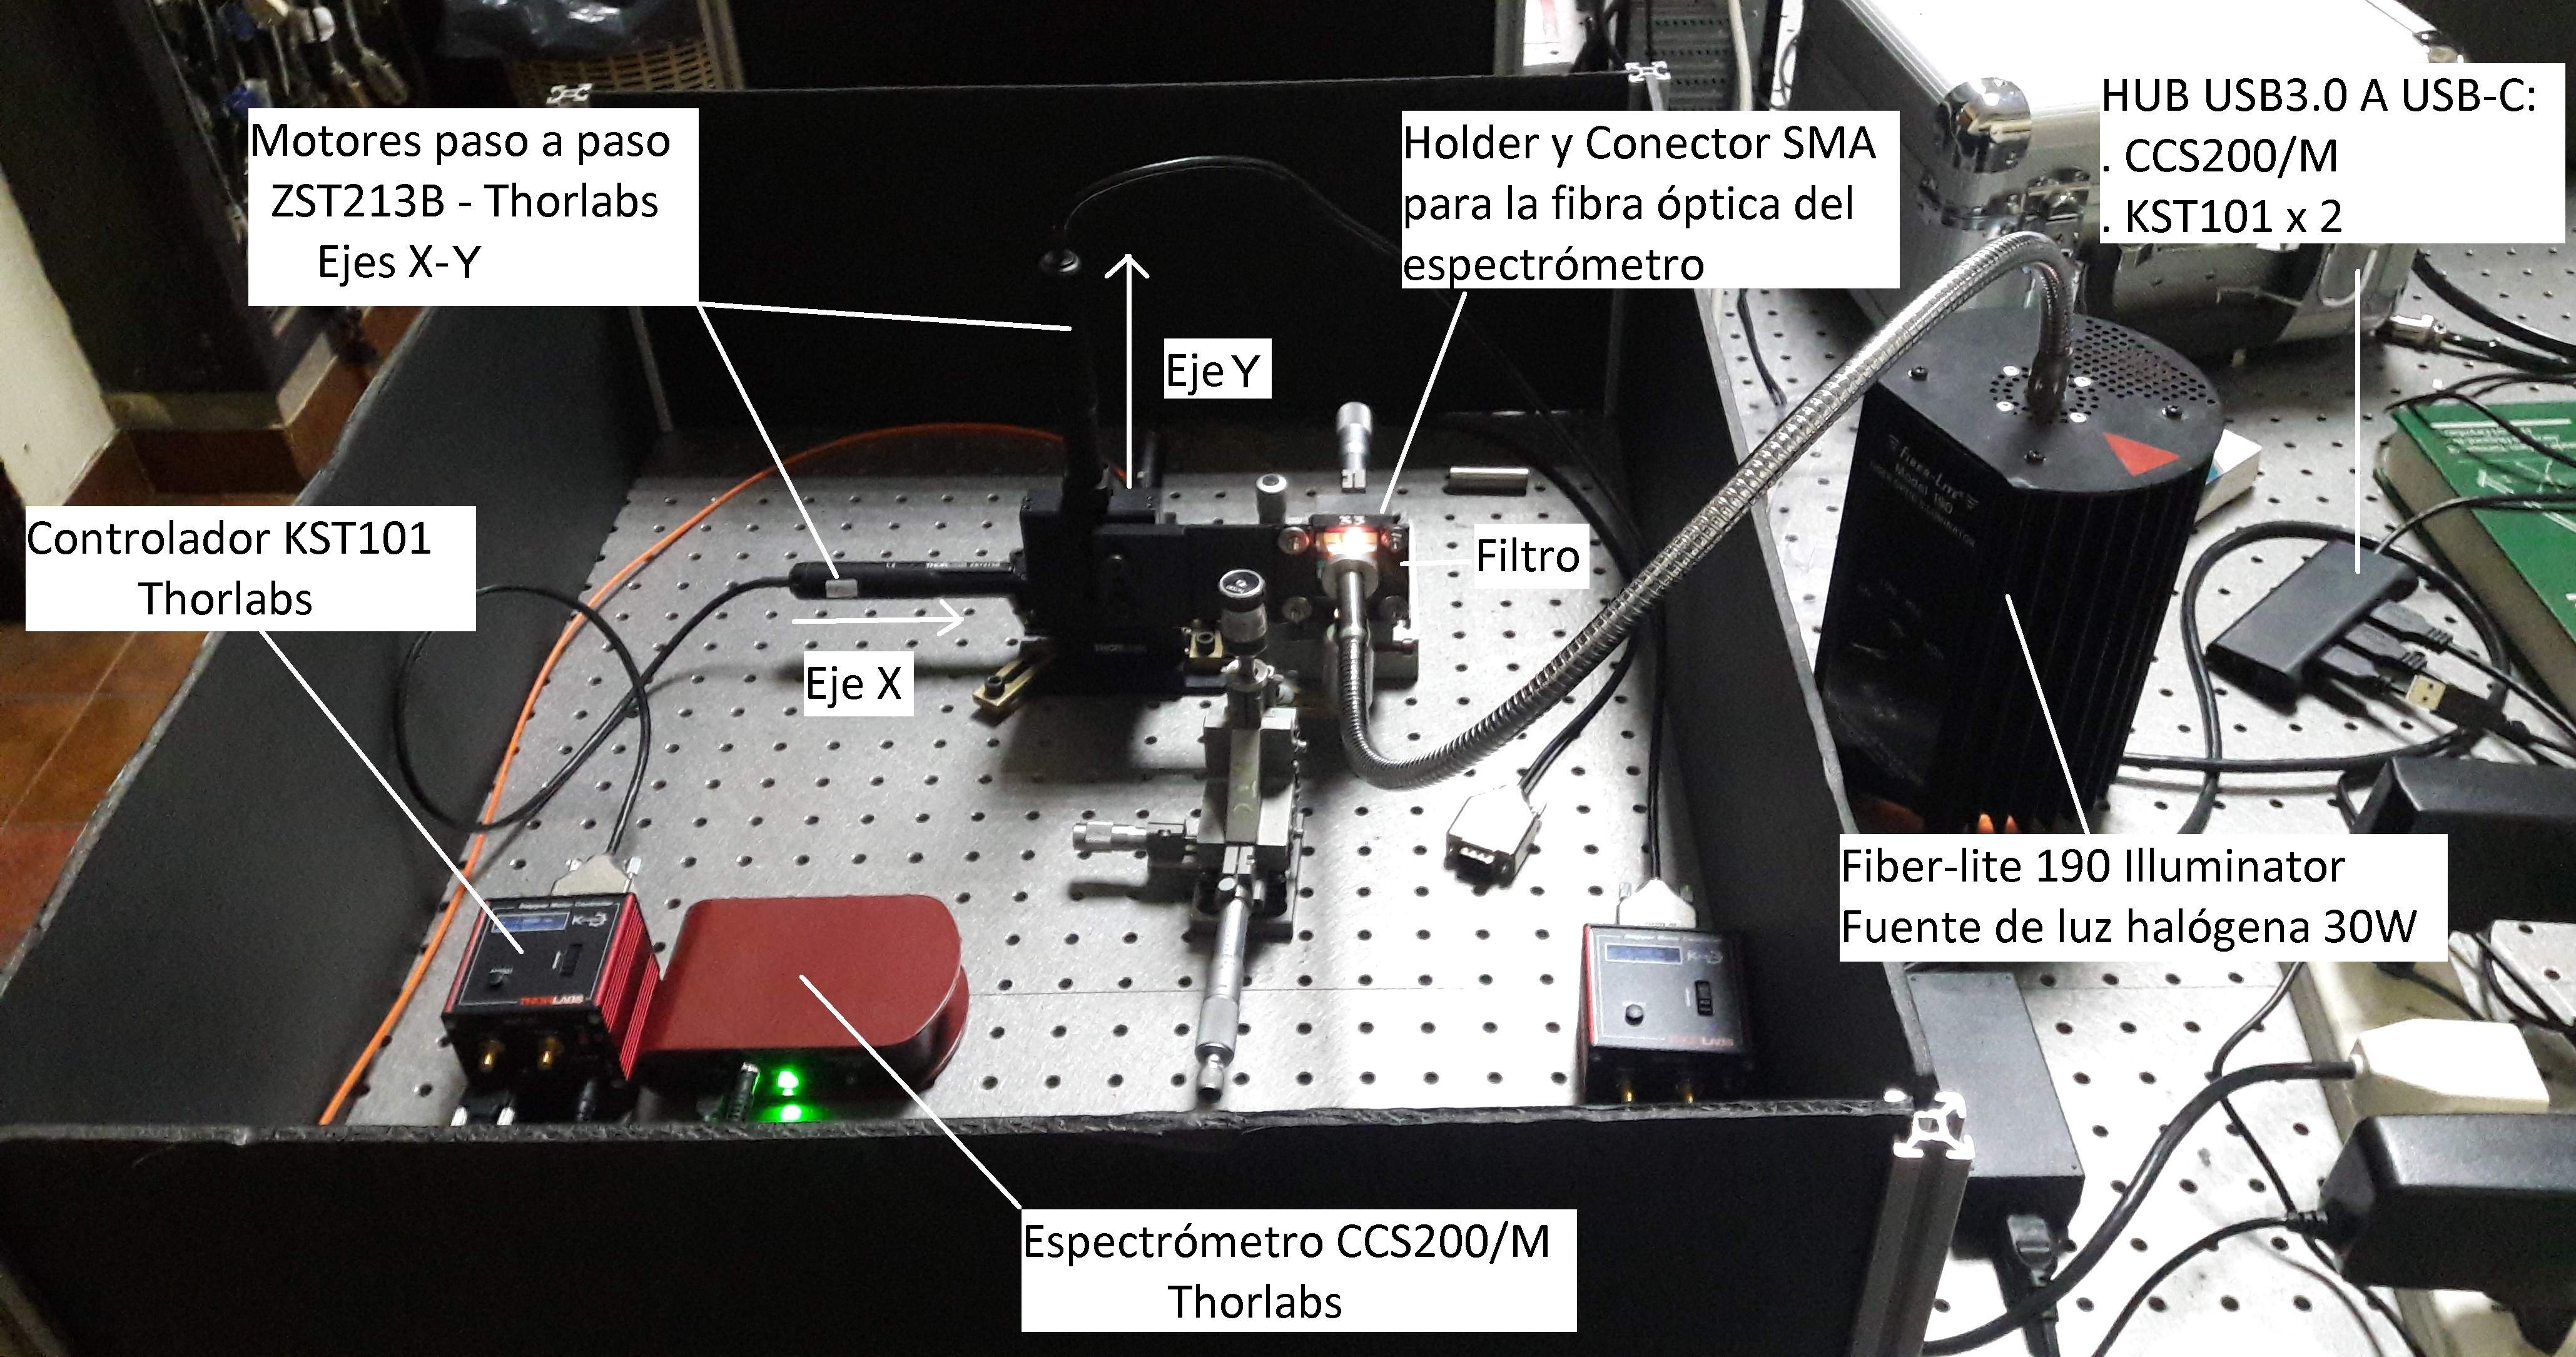
\includegraphics[width=1.0\textwidth]{Figs/microespectrometro/setupbarridooriginal.jpg}
	\caption{Arreglo experimental del prototipo 0.}
	\label{fig:setup0}
\end{figure}

\begin{figure}[H]
	\begin{floatrow}
		\ffigbox{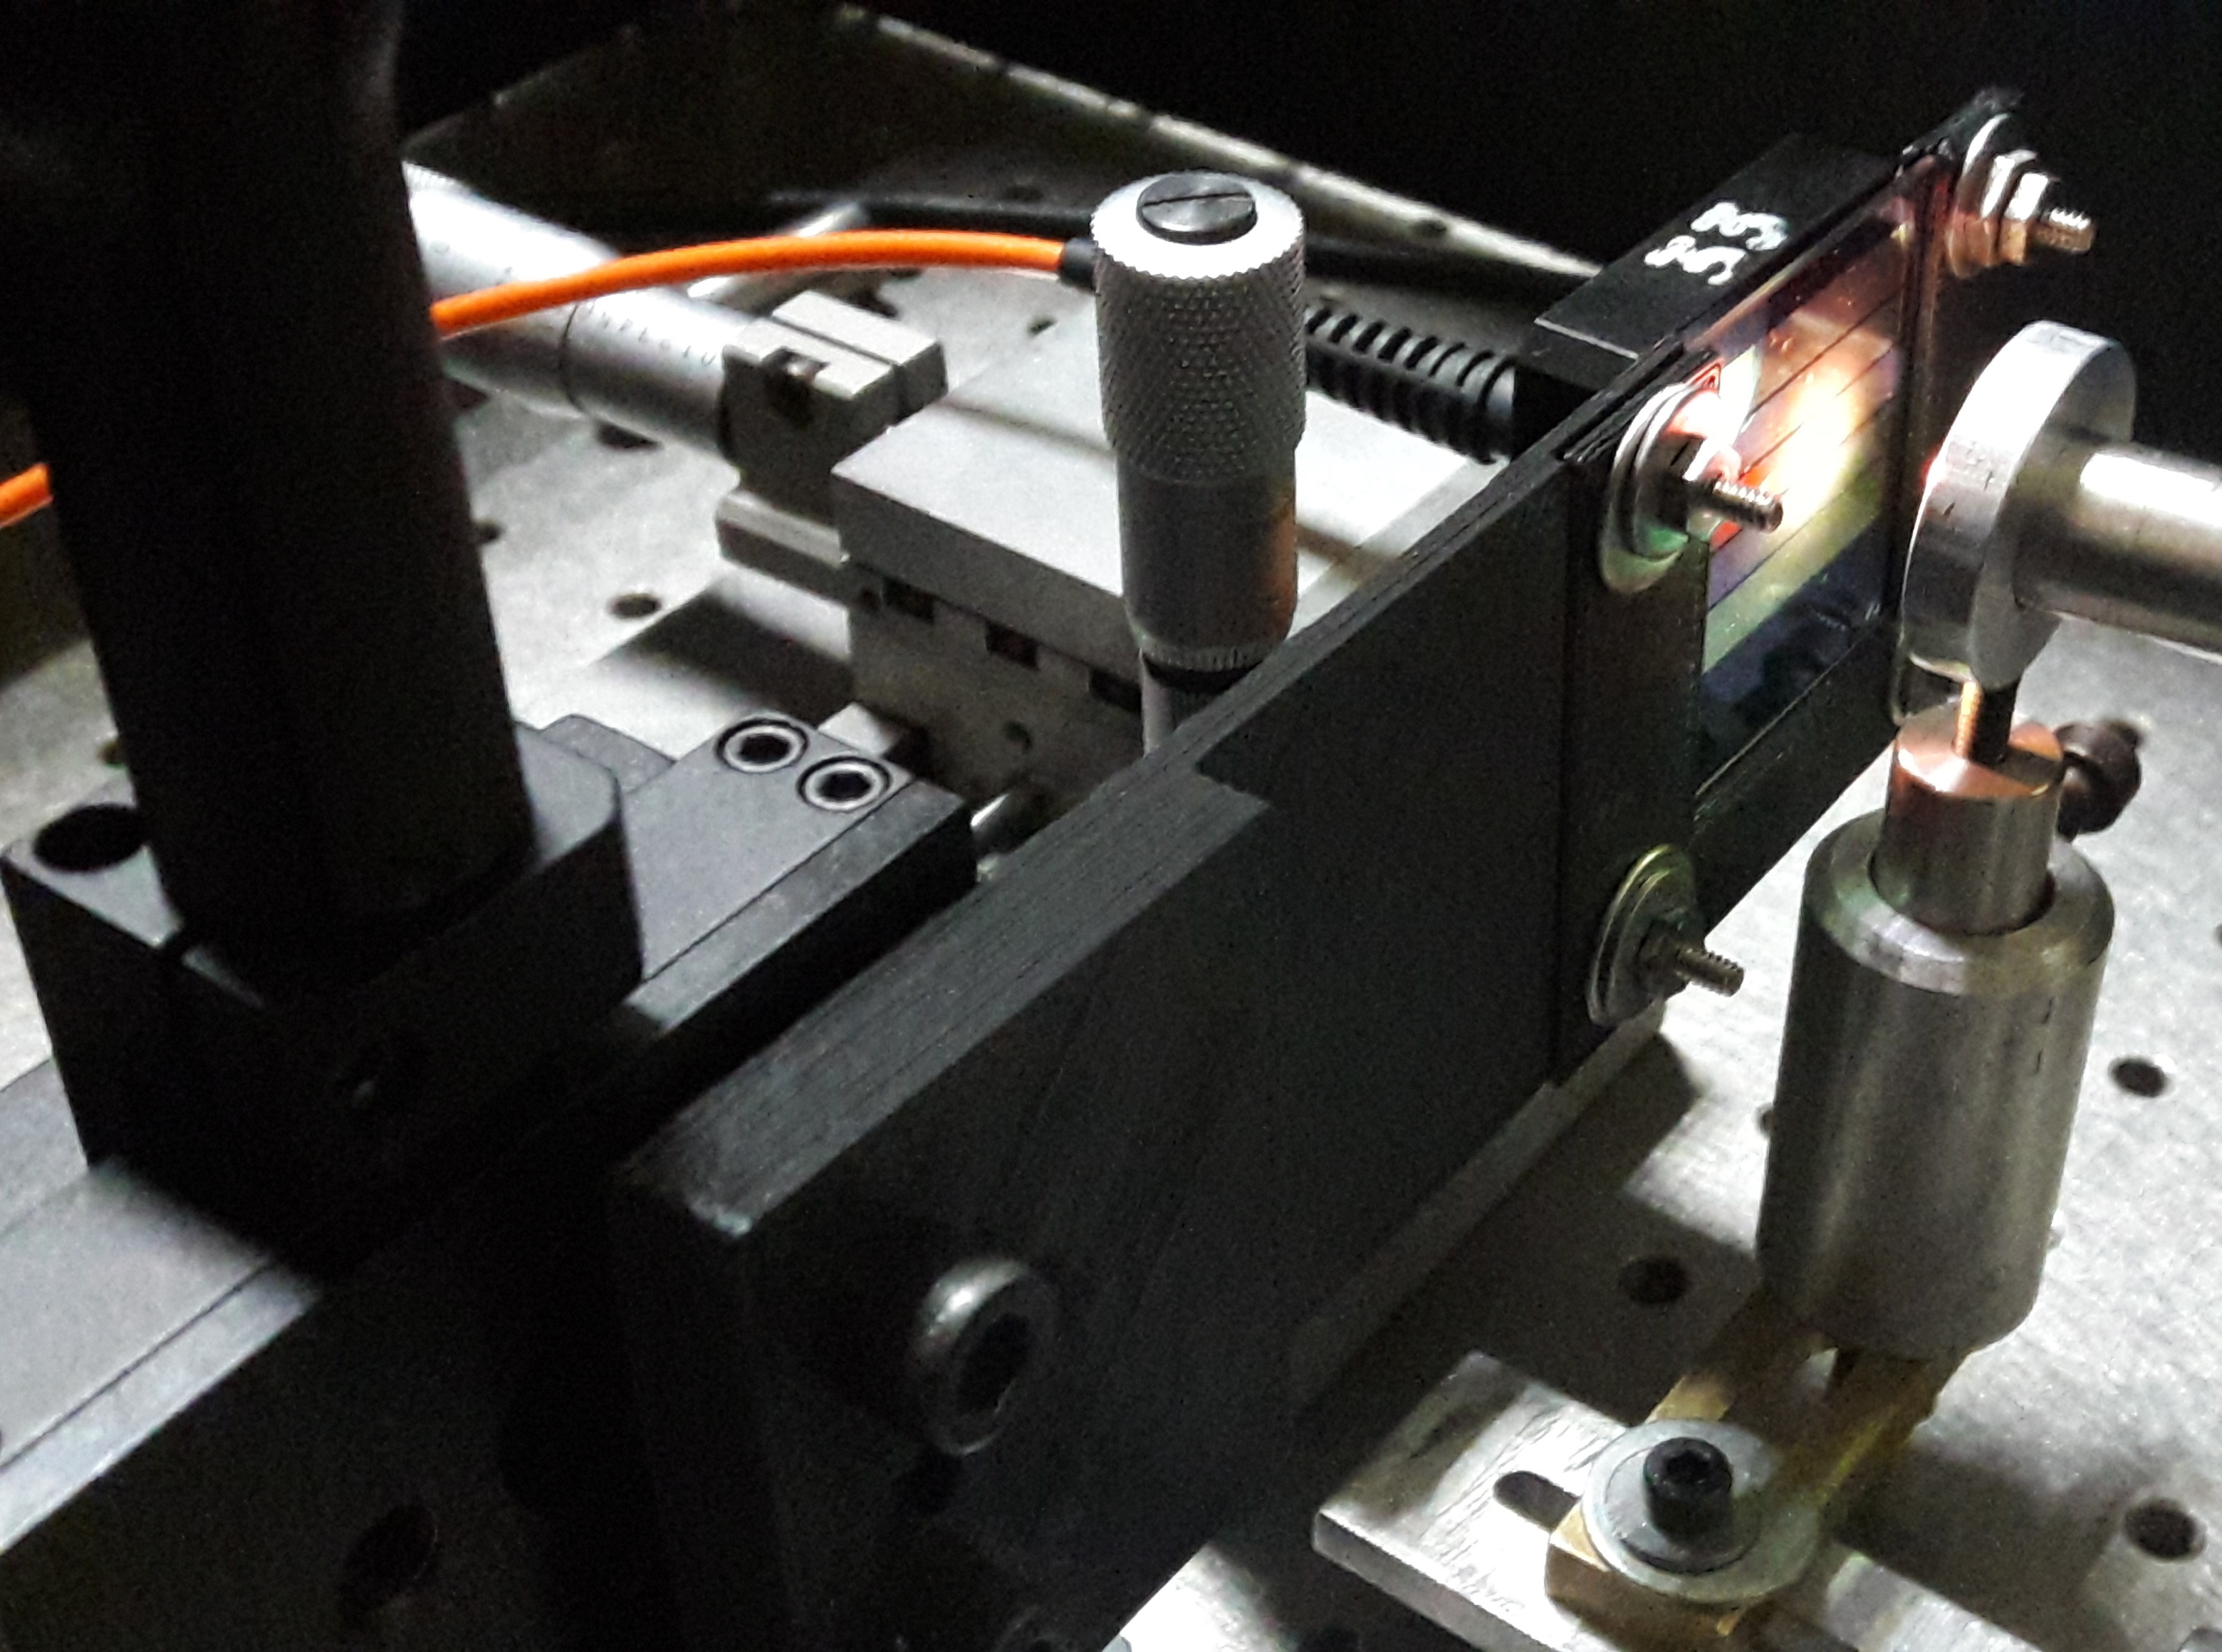
\includegraphics[scale=0.073]{Figs/microespectrometro/montajesetup0.jpg}}{\caption{Vista lateral del montaje del filtro sobre el soporte que se encuentra atornillado con unos tornillos M6 a la plataforma motorizada de Thorlabs.}\label{fig:setup01}}
		\ffigbox{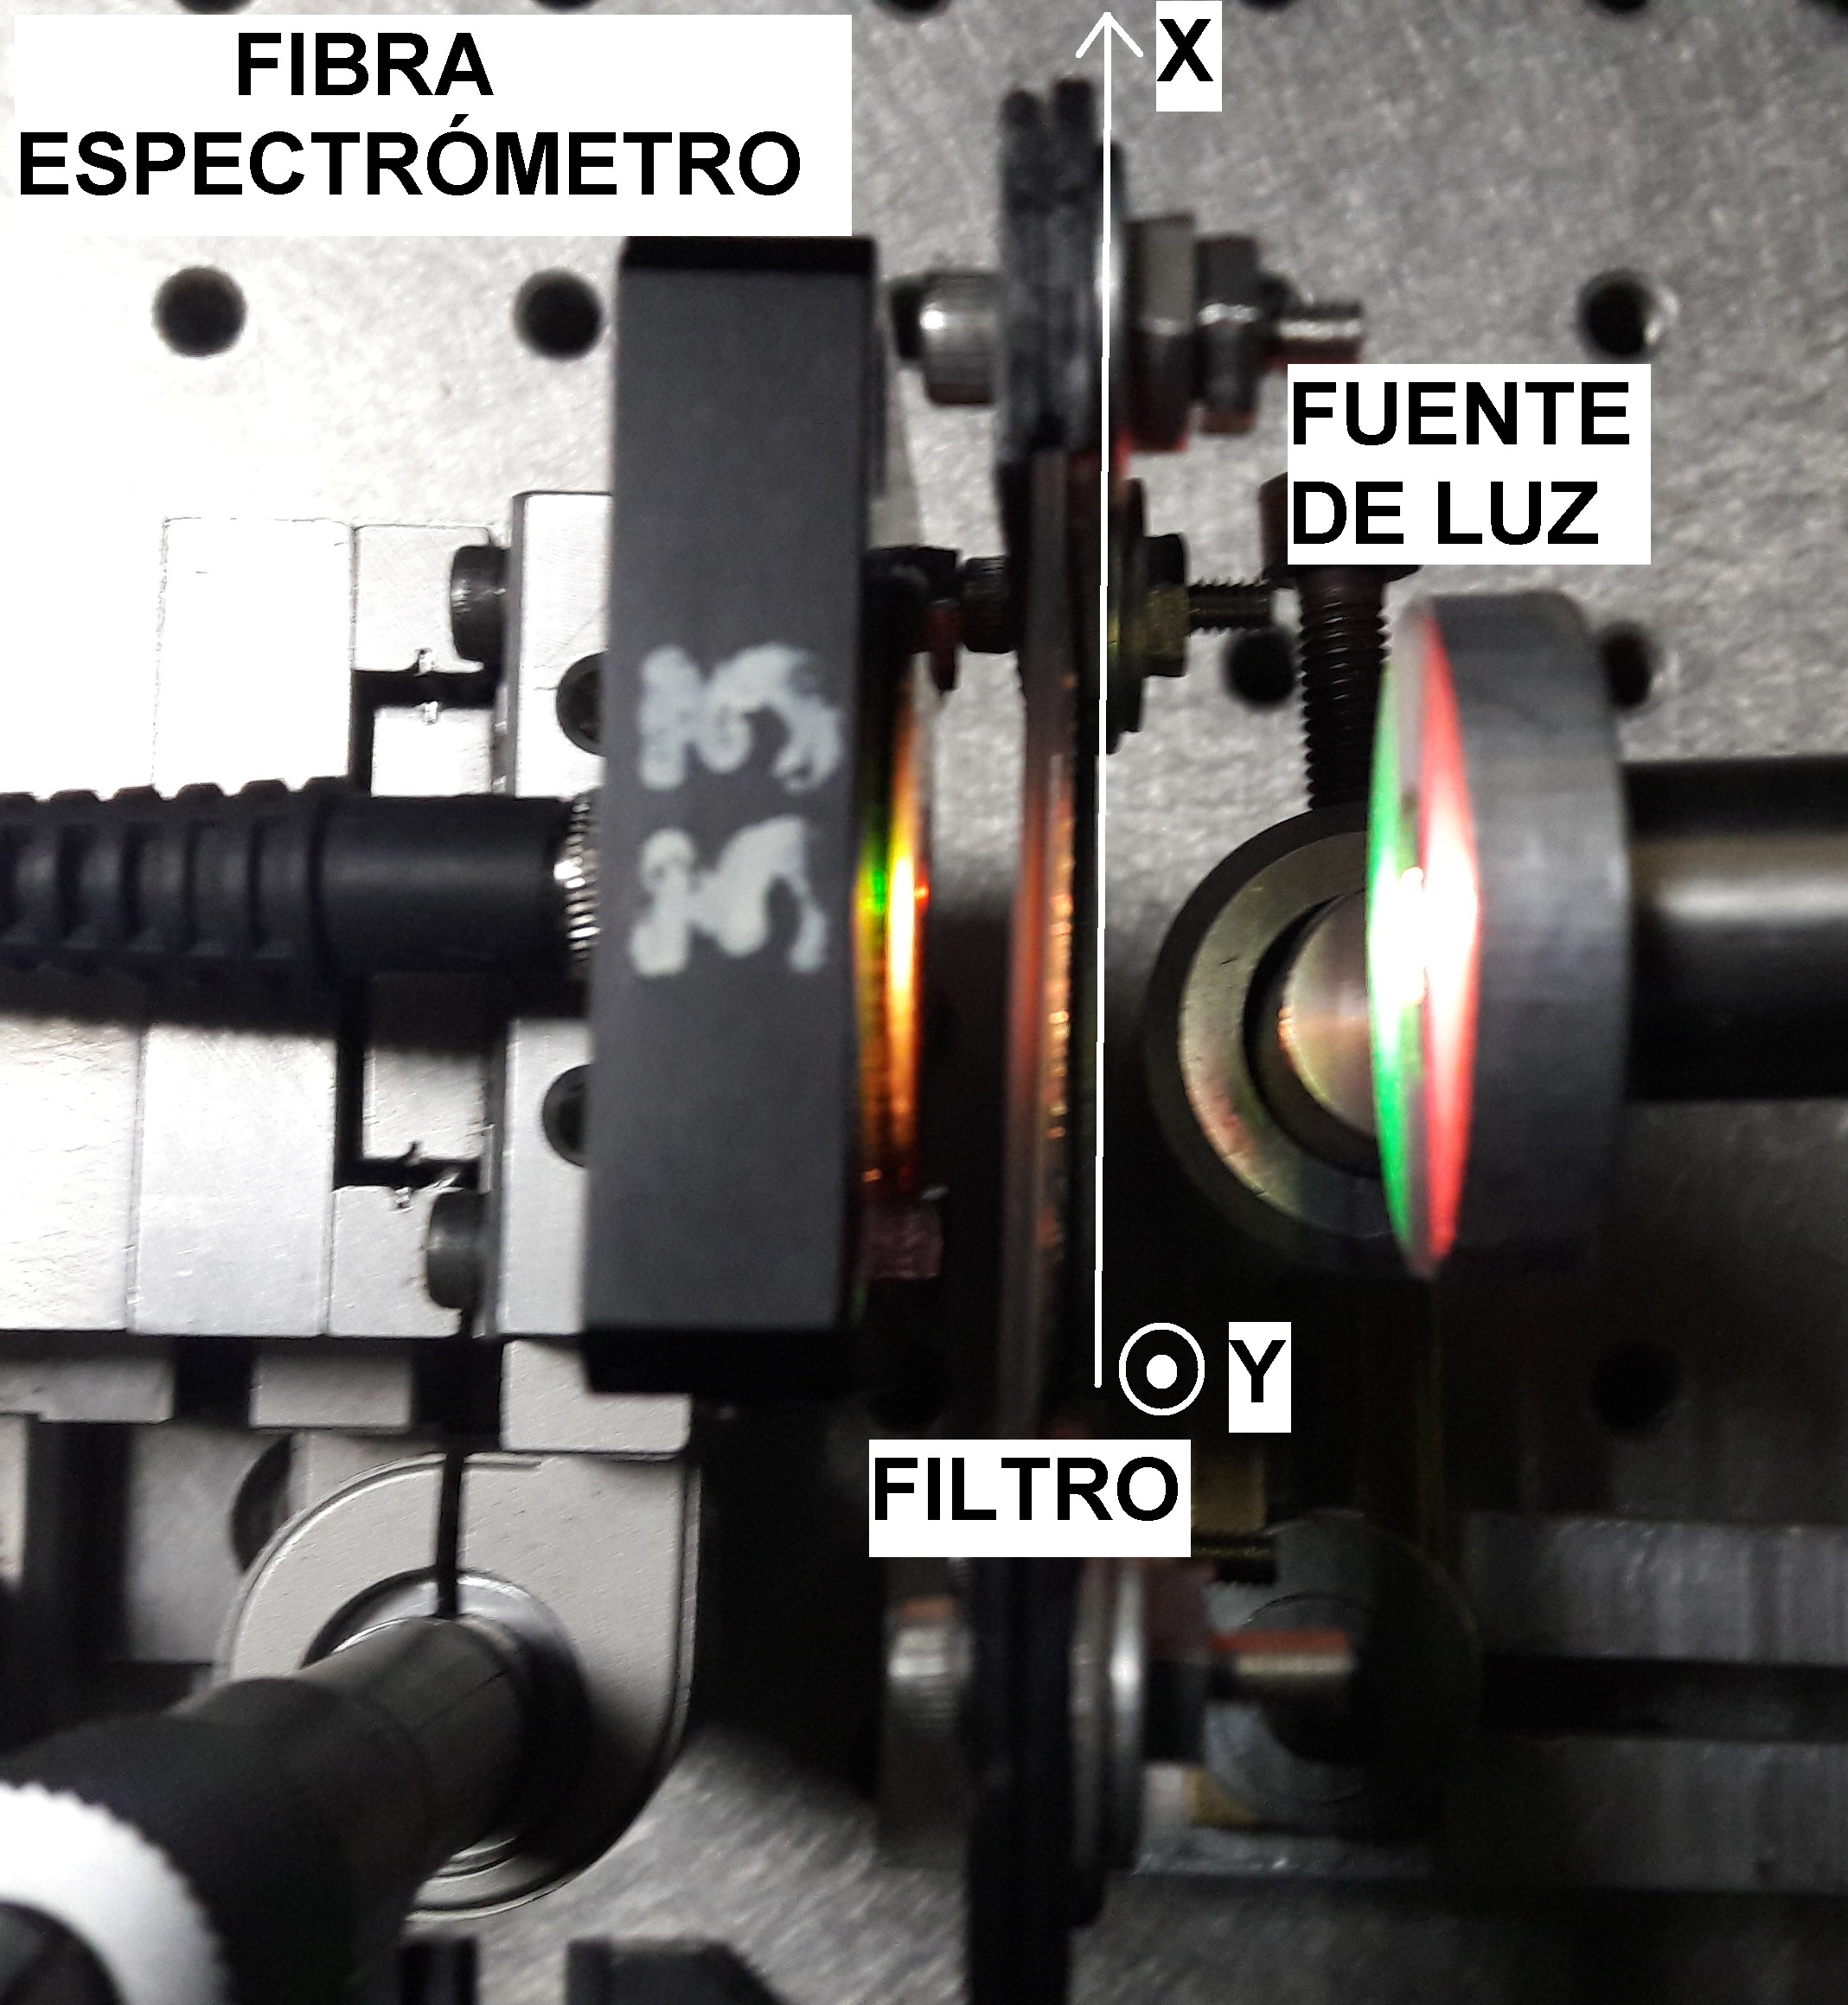
\includegraphics[scale=0.073]{Figs/microespectrometro/5.jpg}}{\caption{El filtro se mueve en los ejes $\textit{x}$ e $\textit{y}$. La fuente de luz y la fibra del espectrómetro se encuentran inmóviles. }\label{fig:setup02}}
	\end{floatrow}
\end{figure}

Con una fuente de luz halógena, modelo \href{https://dolan-jenner.com/products/fiber-lite-190}{\textit{Fiber-lite 190 Illuminator}}, se incidió perpendicularmente sobre el filtro y su transmisión fue detectada por la fibra óptica de un espectrómetro modelo \href{https://www.thorlabs.com/thorproduct.cfm?partnumber=CCS200/M#ad-image-0}{CCS 200/M} de la empresa Thorlabs (\textit{Driver} de \textit{python}: \href{https://github.com/jrr1984/thorlabs_step_motors_ZST213B/blob/master/syst/CCS200.py}{\faGithub}). De la misma manera en que se realizó el \textit{Tile Scan} del filtro completo con el microscopio Zeiss explicado en la sección \ref{subs:tilsc} (Ver Figura \ref{fig:tilescan}), se desplazó el filtro a lo largo del eje x, barriendo en `filas' y realizando el desplazamiento vertical en los extremos del máximo recorrido de los tornillos accionados por los motores paso a paso que fue de 13 mm. Dicho desplazamiento fue realizado con una plataforma de tres grados de libertad, modelo \href{https://www.thorlabs.com/thorproduct.cfm?partnumber=MT3/M}{MT3/M} de la empresa Thorlabs, cuyos tornillos micrométricos fueron intercambiados por unos motores paso a paso modelo \href{https://www.thorlabs.com/thorproduct.cfm?partnumber=ZST213B}{ZST213B} cuyos controladores fueron también de la empresa Thorlabs, modelo \href{https://www.thorlabs.com/thorproduct.cfm?partnumber=KST101}{KST101} (\textit{Driver} de \textit{python}: \href{https://github.com/jrr1984/thorlabs_step_motors_ZST213B/blob/master/barrido/std/thor_stepm.py}{\faGithub}). Como las dimensiones de la región comprendida por las cinco bandas del filtro es de 27 mm x 25 mm, con esta plataforma no se pudo realizar una adquisición del filtro completa en una sola configuración como la propuesta. El \textit{software} automatizado de adquisición del espectro de transmisión del filtro desarrollado para este prototipo [\href{https://github.com/jrr1984/thorlabs\_step\_motors\_ZST213B/tree/master/barrido/std}{\faGithub}] fue expandido en el prototipo final y se lo explica en la Sección \ref{sec:softadq}.


No se utilizó ningún arreglo óptico ni para enfocar la fuente de luz en el filtro ni para enfocar su transmisión divergente sobre la fibra óptica del espectrómetro. No se caracterizó la resolución óptica con la que se realizaron las mediciones con el espectrómetro en este prototipo ni el tamaño del objeto medido sobre la superficie del filtro. La resolución óptica y magnificación necesarias para medir los defectos del filtro fueron establecidas a partir de los resultados del Capítulo \ref{chap:zeiss} y fueron consideradas en el diseño óptico del microespectrómetro desarrollado que se explica en la Sección \ref{sec:disop}.


Respecto del segundo objetivo específico propuesto relacionado con la determinación de un mapa de colores ($\textit{x}$,$\textit{y}$,$\lambda$) del filtro, se adquirió el espectro de transmisión del filtro en dos barridos cuyas dimensiones fueron de 13 mm a lo largo del eje $\textit{x}$ y de 12.2 mm a lo largo del eje $\textit{y}$, definidos de acuerdo a la Figura \ref{fig:setup02}. La adquisición fue realizada en dos etapas debido a la limitación del recorrido de los tornillos desplazados por los motores paso a paso como se explicó anteriormente. De esta manera se adquirió en primer lugar la región superior del filtro que contiene a las bandas azul, verde y parte de la pancromática con una cierta altura de la fuente de luz y de la fibra del espectrómetro. La fuente y la fibra se encontraban montadas sobre unos posicionadores micrométricos con los cuales se varió su altura respecto del filtro para poder medir la región inferior del filtro que contenía la región faltante de la banda pancromática, la banda roja y la banda del NIR. En la F









\singlespacing
\section{Montaje y construcción de un microespectrómetro}
\label{sec:montcontmsp}
\spacing{1.5}

\singlespacing
\subsection{Fuente de luz y espectrómetro}
\label{sec:fteluzyesp}
\spacing{1.5}

\singlespacing
\subsection{Platina}
\label{sec:platina}
\spacing{1.5}

\singlespacing
\subsection{Diseño óptico del microespectrómetro}
\label{sec:disop}
\spacing{1.5}

\singlespacing
\subsection{Montaje y alineación preliminar del microespectrómetro}
\label{sec:montalin}
\spacing{1.5}

\singlespacing
\subsection{Foco y resolución espacial del microespectrómetro}
\label{sec:focoresol}
\spacing{1.5}

\hspace{0.5cm}Para poner en foco el microespectrómetro sobre la cara externa del filtro más cerca al objetivo, se buscó el mínimo de la resolución espacial.

La resolución espacial se obtiene a partir del ajuste de las mediciones de una transición banda-cromo.

Para no alargar el tiempo de duración de las mediciones se mapeó el espectrómetro con la cámara. De lo contrario el único feedback que se tiene para saber si se está en una banda o en el cromo es la medición del espectro.

En consecuencia se conectó la fibra óptica montada sobre el cage destinado a medir con el espectrómetro, a la fuente de luz y por reflexión se observó en la adquisición en vivo de la cámara en qué posición de la imagen se observaba el haz de luz reflejado. Se centró dicho haz al centro de la cámara y de esa forma se determinó que el centro de la cámara está asociado con la medición efectiva del microespectrómetro. Se hace notar que la cámara no se encuentra en foco todavía, solo fue puesta aproximadamente a la misma distancia focal que la lente de tubo.

El setup para realizar este mapeo es el siguiente:
\begin{figure}[H]
	\centering
	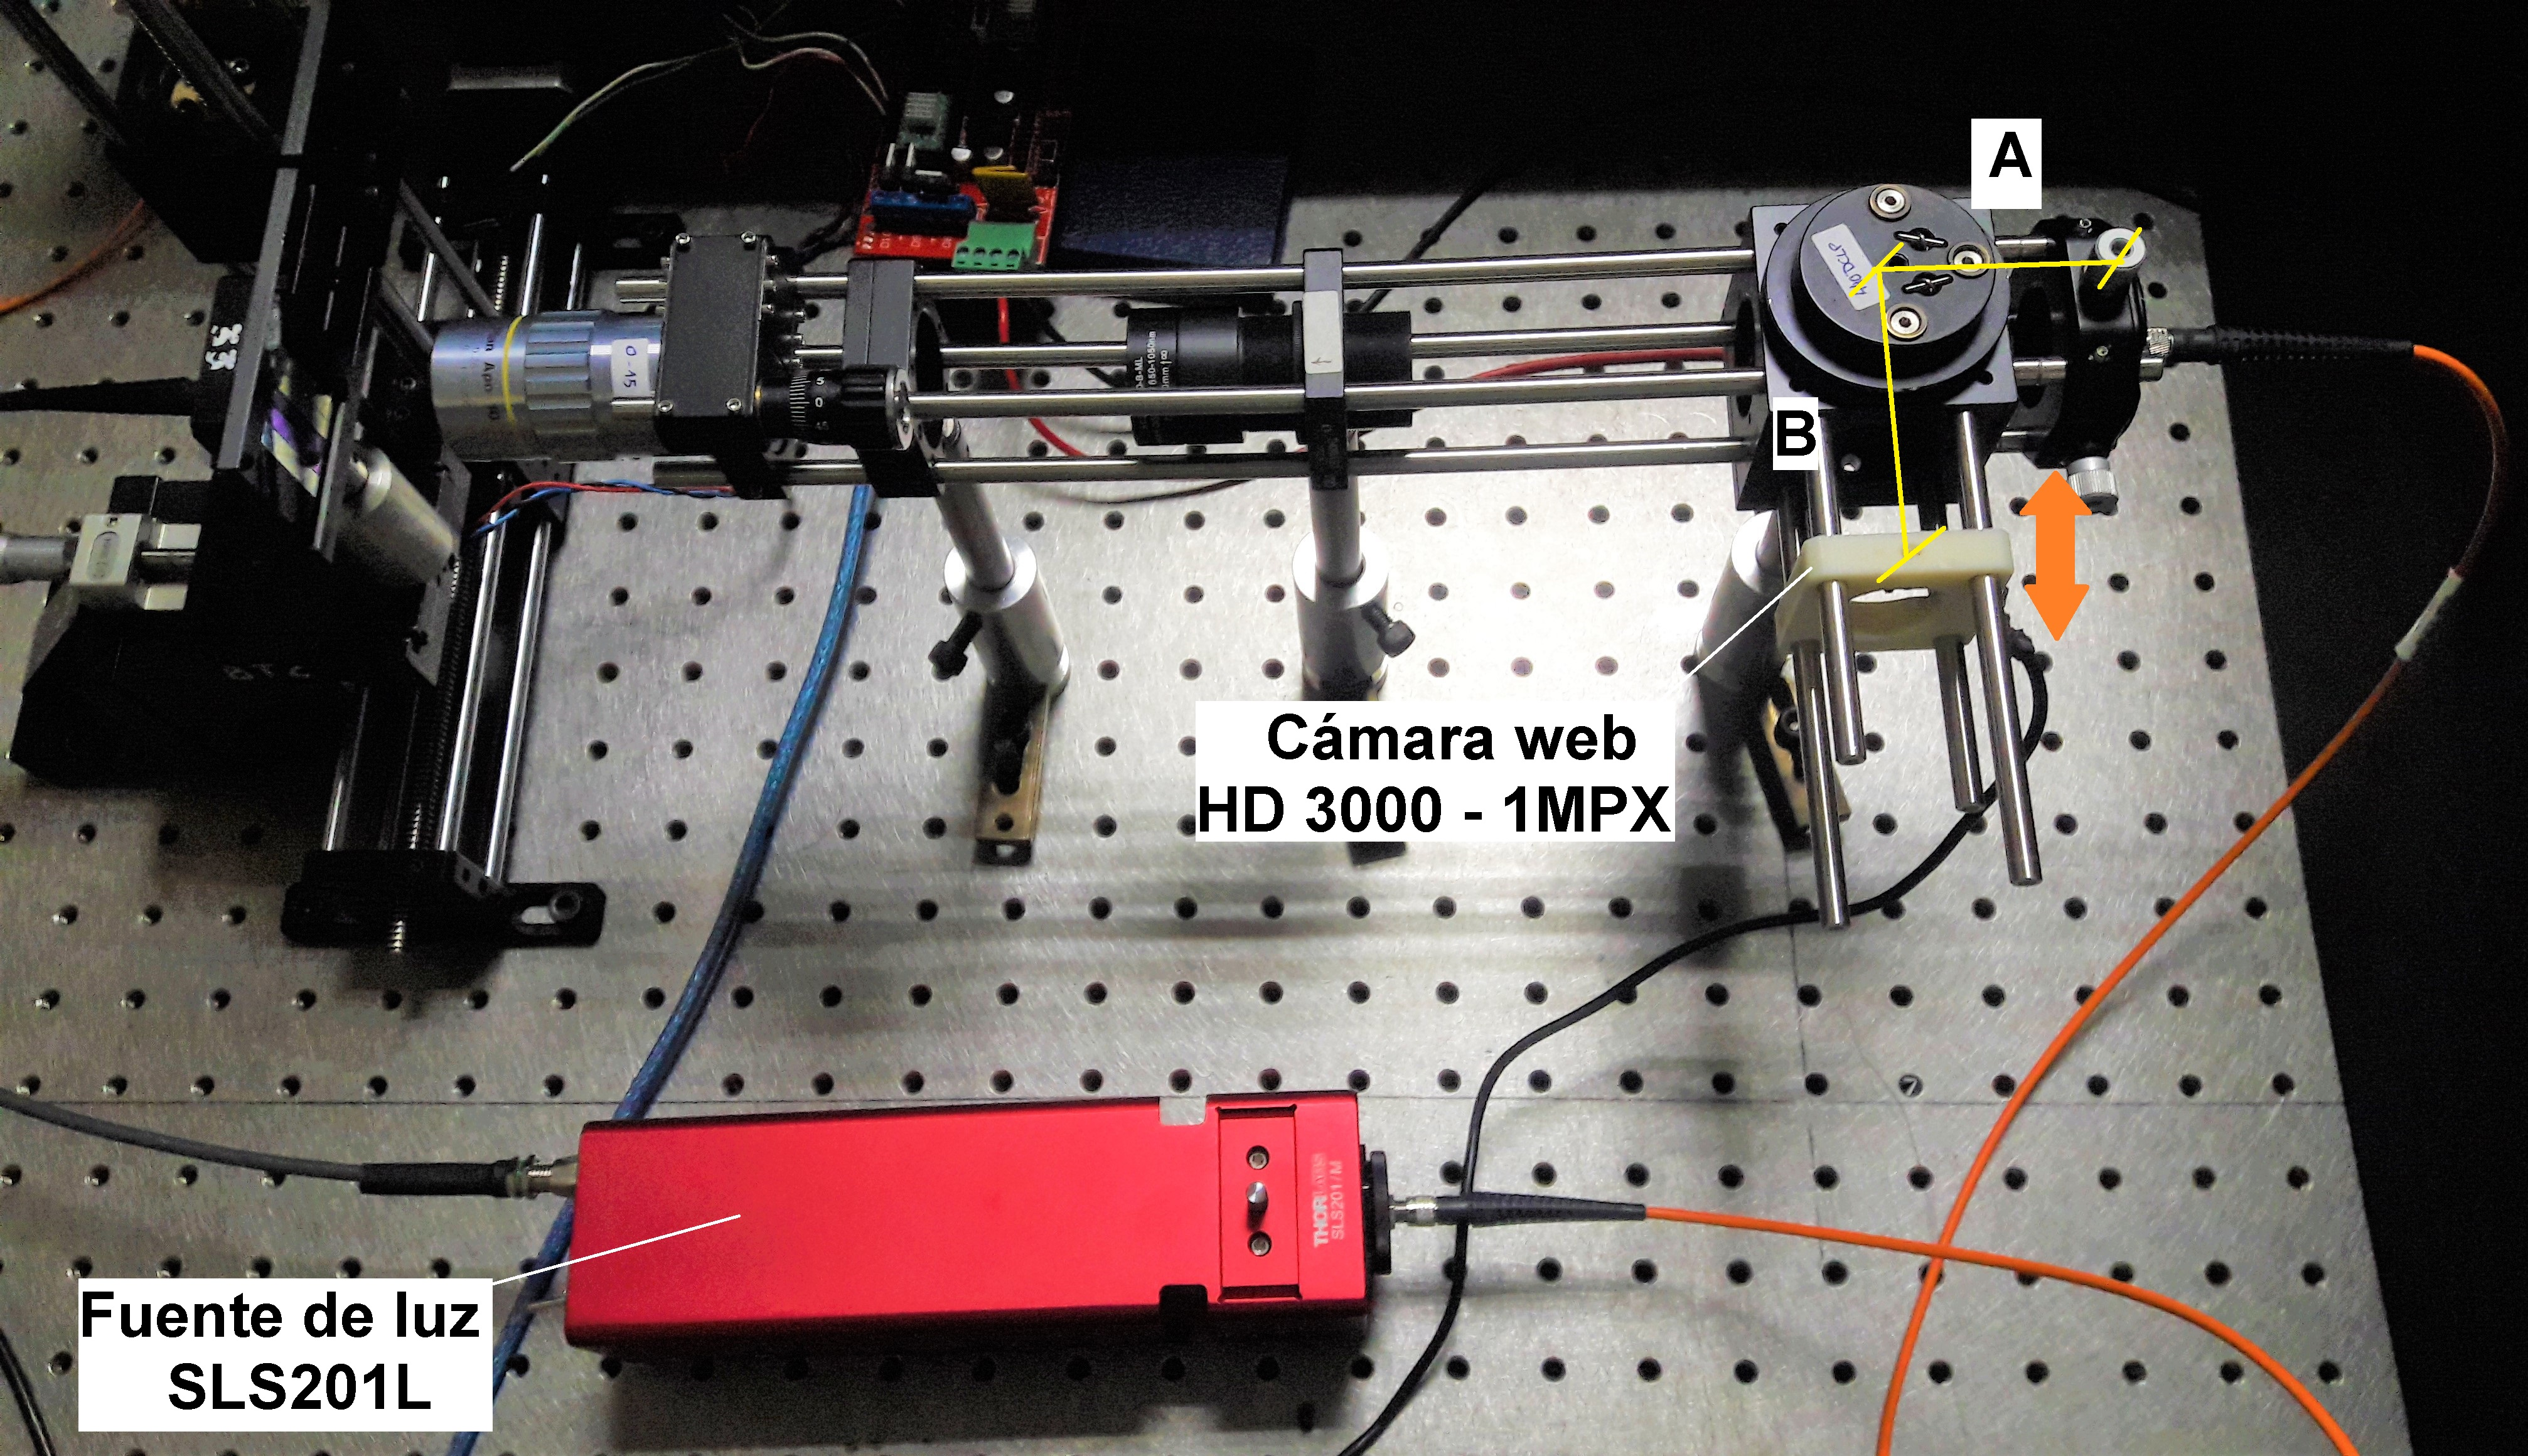
\includegraphics[scale=0.1]{Figs/microespectrometro/mapespeccam.jpg}
	\caption{Setup para mapear el espectrómetro con la cámara.}
	\label{fig:bgcel}
\end{figure}


Con los tornillos de la tapa de arriba del beamsplitter se puede ajustar en altura el beamsplitter para poder observar en el centro de la cámara la medición del espectrómetro.
\begin{figure}[H]
	\centering
	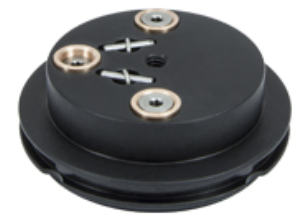
\includegraphics[scale=0.5]{Figs/microespectrometro/b4c.png}
	\caption{Tapa de arriba del beamsplitter.}
	\label{fig:bgcel}
\end{figure}


\begin{figure}[H]
	\centering
	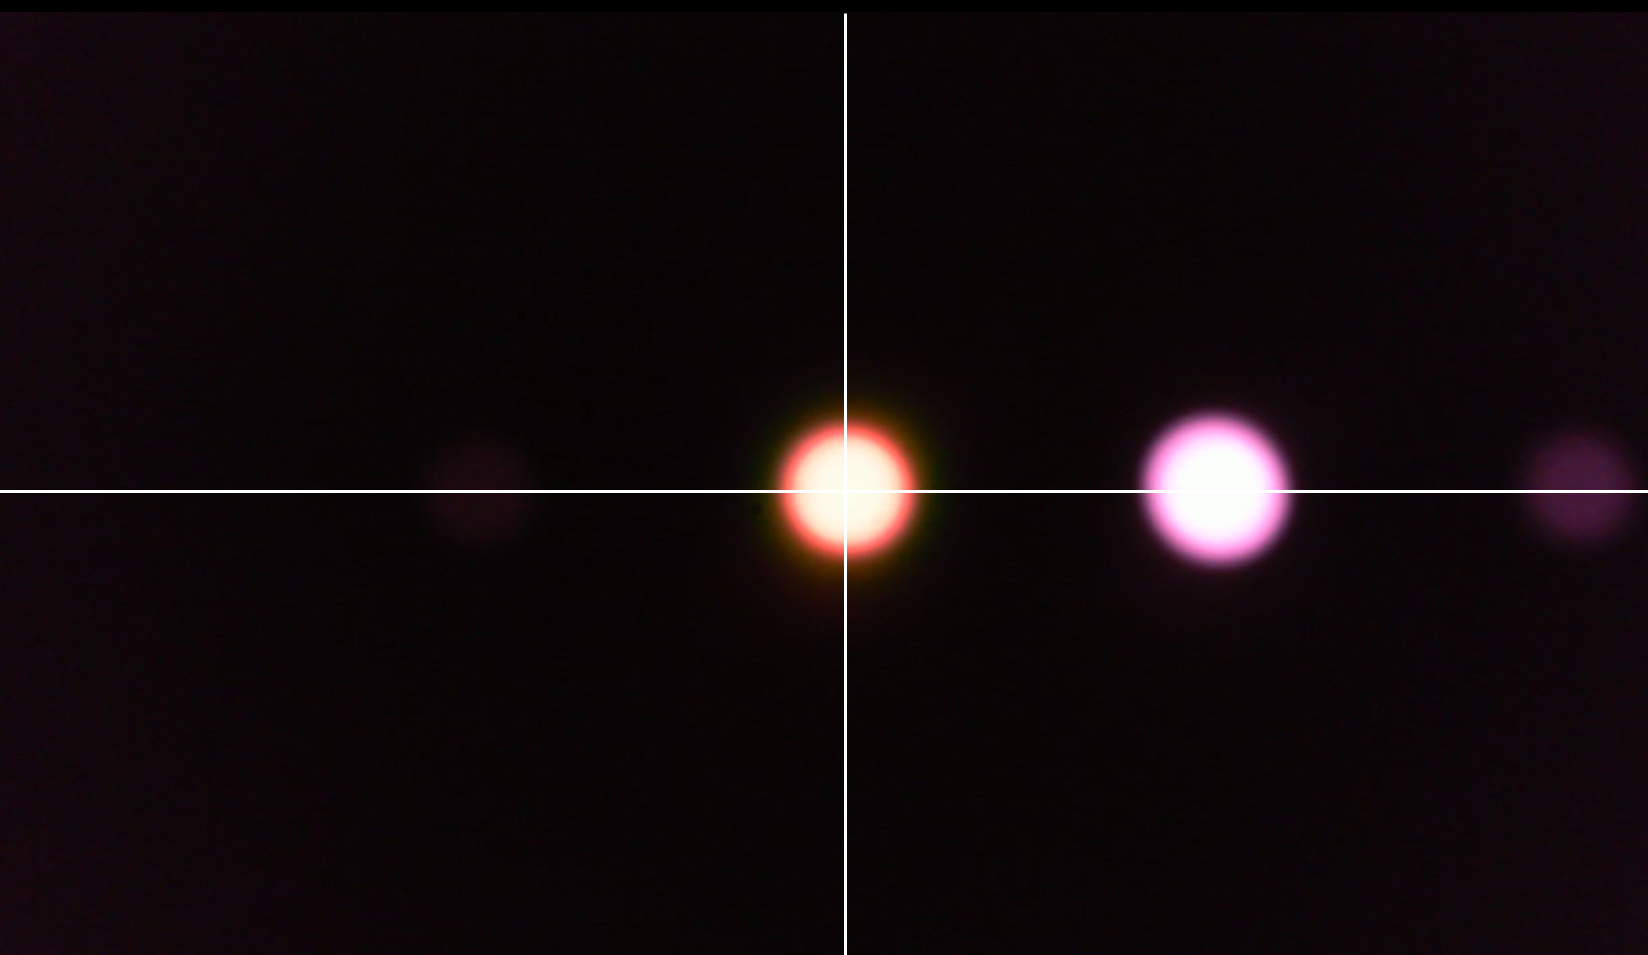
\includegraphics[scale=0.5]{Figs/microespectrometro/mapspectrometrocamera.png}
	\caption{Visualización en la cámara de la reflexión del filtro de la iluminación.}
	\label{fig:bgcel}
\end{figure}


No se tocó ni la cámara ni ninguna parte del setup a partir de ese momento para no perder este mapeo, a pesar de que la cámara no se encuentre perfectamente en foco (no hace falta probablemente poner una imagen de la cámara mostrando que no está en foco..), es decir que la imagen no se vea del todo nítida.
Luego se puso en foco el microespectrómetro.



\begin{figure}[H]
	\centering
	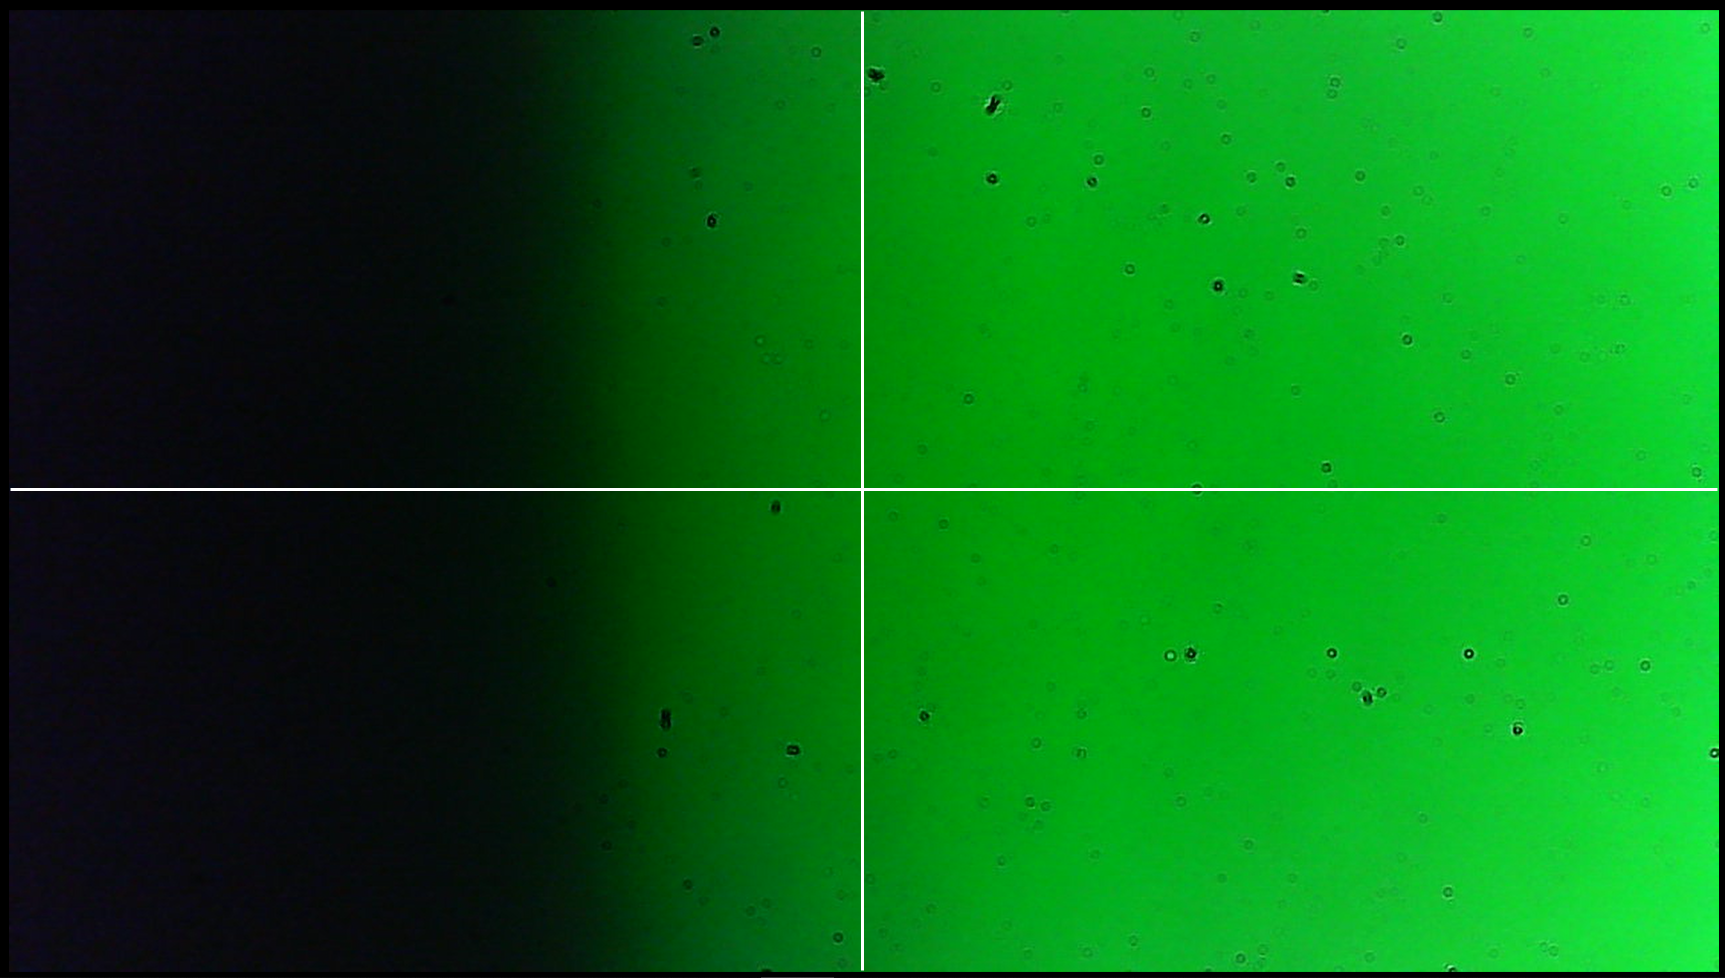
\includegraphics[scale=0.5]{Figs/microespectrometro/medtransicion.png}
	\caption{Visualización en la cámara de la reflexión del filtro de la iluminación.}
	\label{fig:bgcel}
\end{figure}


durante el experimento se tiene el feedback de cutelog:

\begin{figure}[H]
	\centering
	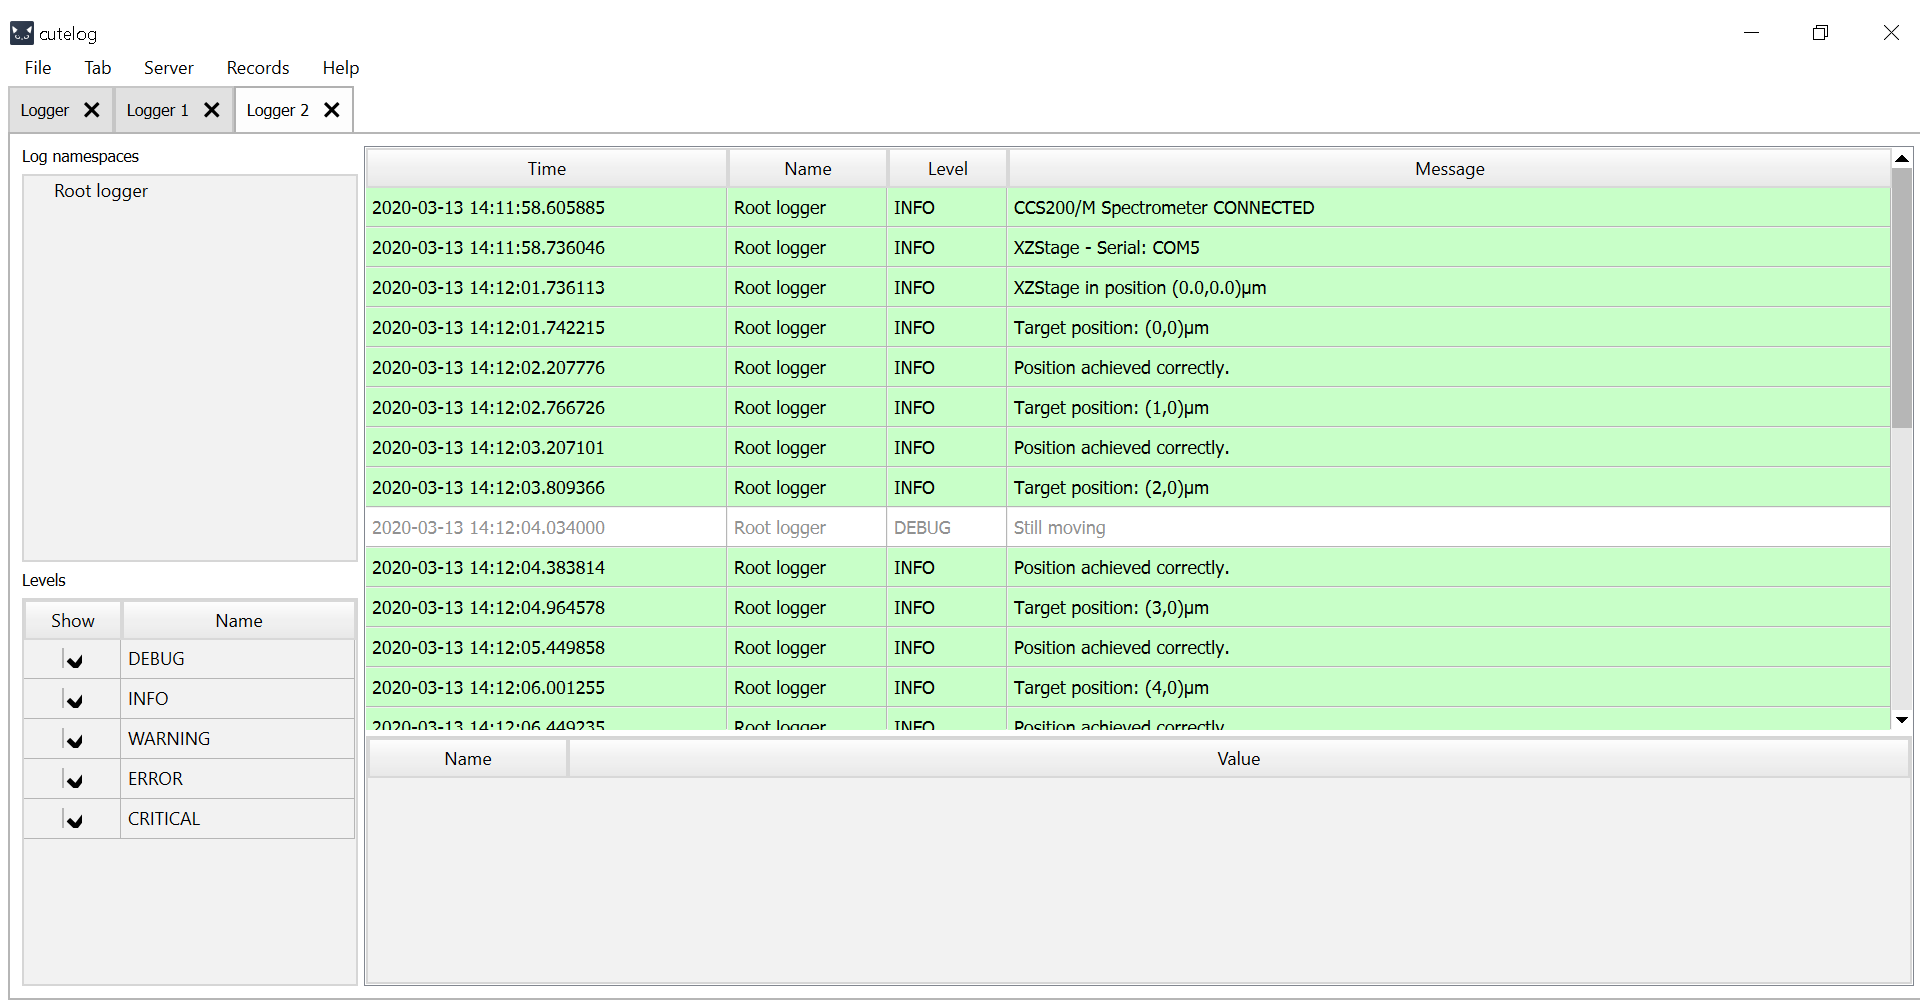
\includegraphics[scale=0.5]{Figs/microespectrometro/cutelog.png}
	\caption{Visualización en la cámara de la reflexión del filtro de la iluminación.}
	\label{fig:bgcel}
\end{figure}


\begin{figure}[H]
	\centering
	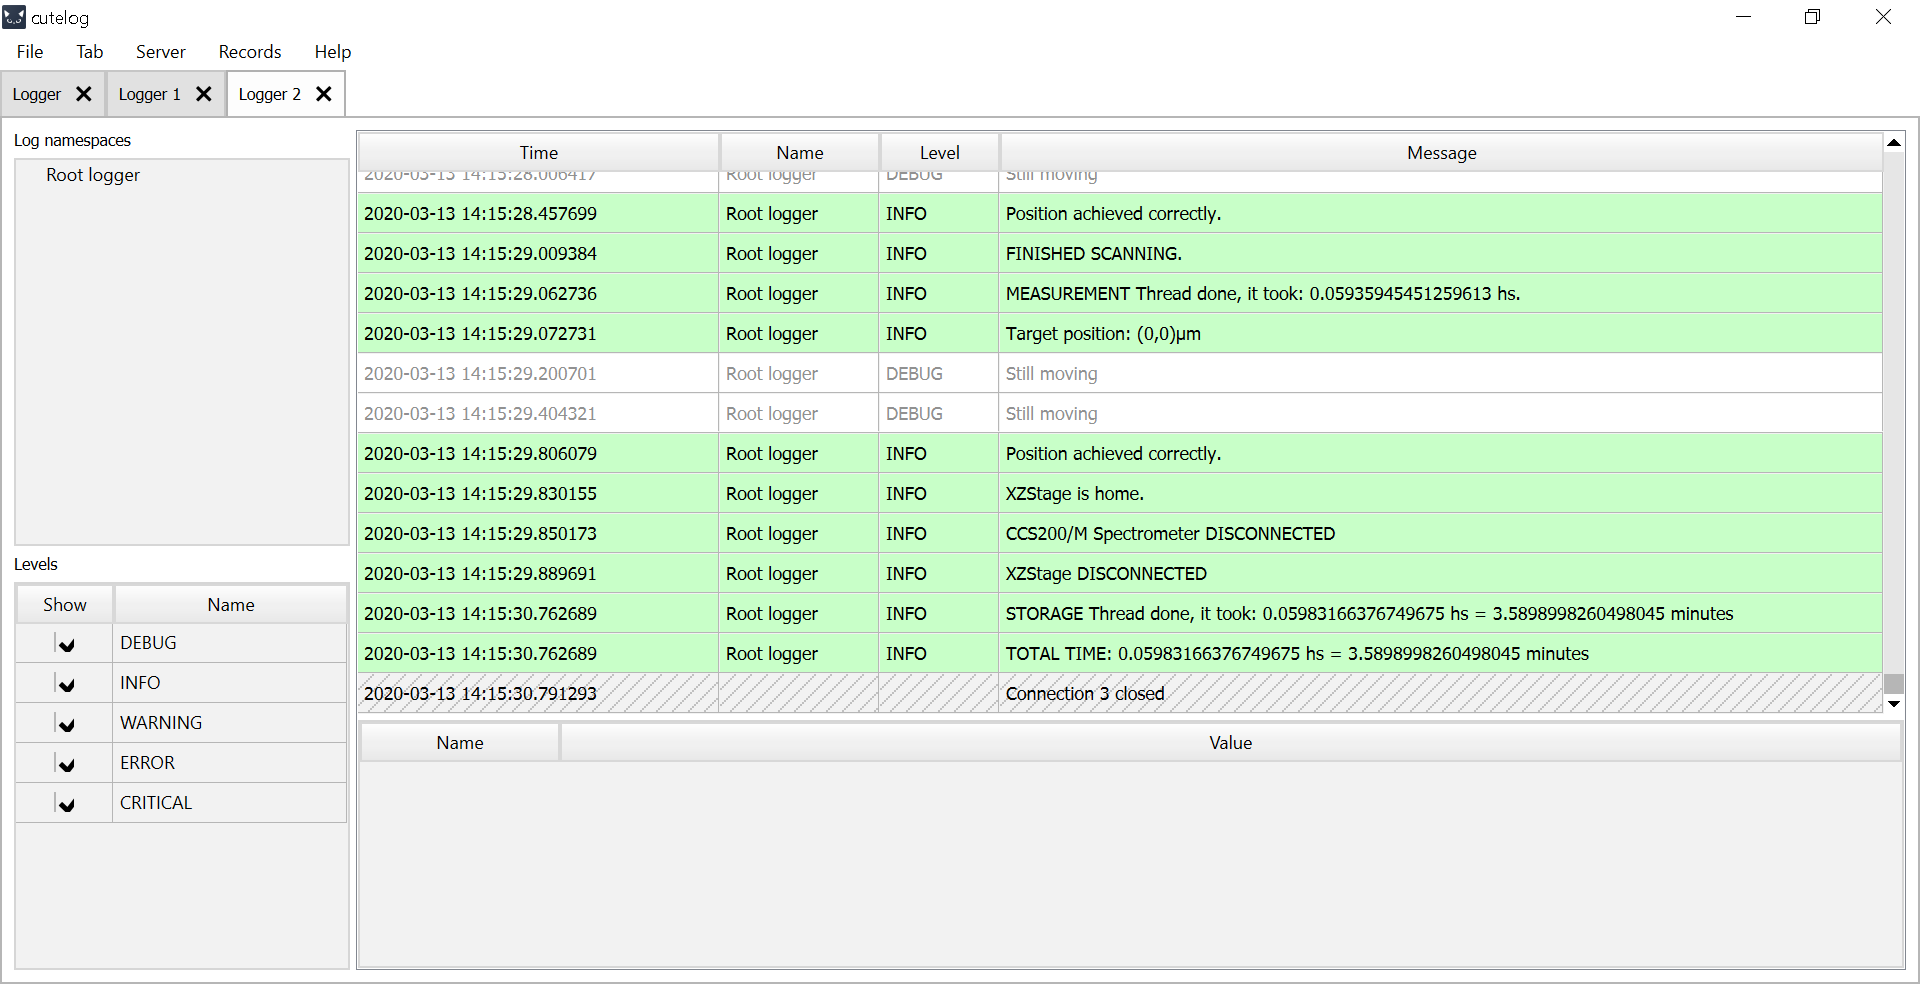
\includegraphics[scale=0.5]{Figs/microespectrometro/fincutelog.png}
	\caption{Visualización en la cámara de la reflexión del filtro de la iluminación.}
	\label{fig:bgcel}
\end{figure}


Las mediciones son ajustadas en matlab con una función error:
\begin{equation}
	(a/2)*erfc(sqrt(2)*(x-b)/c)
\end{equation}

\begin{figure}[H]
	\centering
	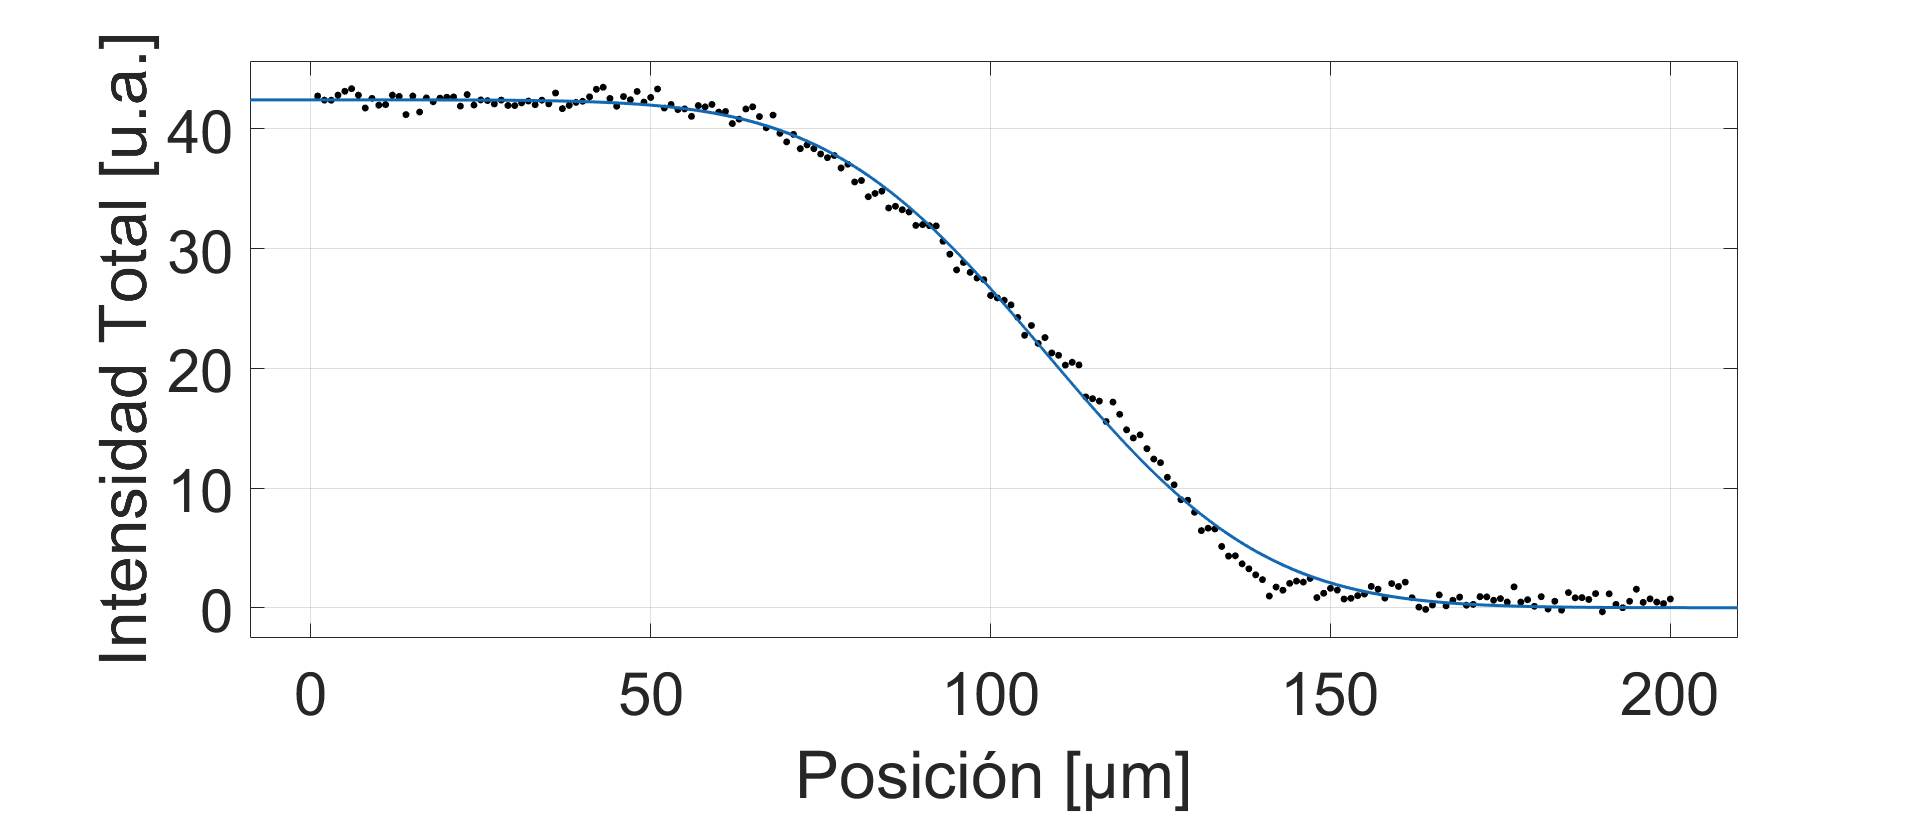
\includegraphics[scale=0.3]{Figs/microespectrometro/fit0.png}
	\caption{Visualización en la cámara de la reflexión del filtro de la iluminación.}
	\label{fig:bgcel}
\end{figure}

Resultados del ajuste:

General model:\par
$f(x) = (a/2)*erfc(sqrt(2)*(x-b)/c)$ \par
Coefficients (with 95$\%$ confidence bounds): \par
$a =       42.43  (42.2, 42.66)$\par
$b =       108.2  (107.8, 108.7)$\par
$c =       50.46  (49.25, 51.68)$\par

Goodness of fit:\par
SSE: 151.1\par
R-square: 0.9976\par
Adjusted R-square: 0.9976\par
RMSE: 0.8758\par

Luego moviendo la perilla del SM1Z para cambiar la distancia entre el objetivo y el filtro se repite la medición.


Comentar bien la siguiente foto, poner en la imagen que distancia se está variando, ettc
\begin{figure}[H]
	\centering
	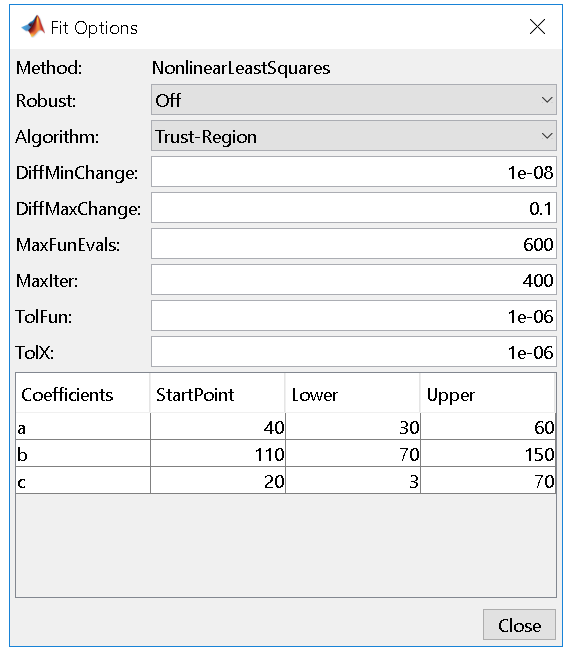
\includegraphics[scale=0.4]{Figs/microespectrometro/refinacionparam.png}
	\caption{Visualización en la cámara de la reflexión del filtro de la iluminación.}
	\label{fig:bgcel}
\end{figure}


Para hacer el ajuste se refinan los parámetros del modelo:

\begin{figure}[H]
	\centering
	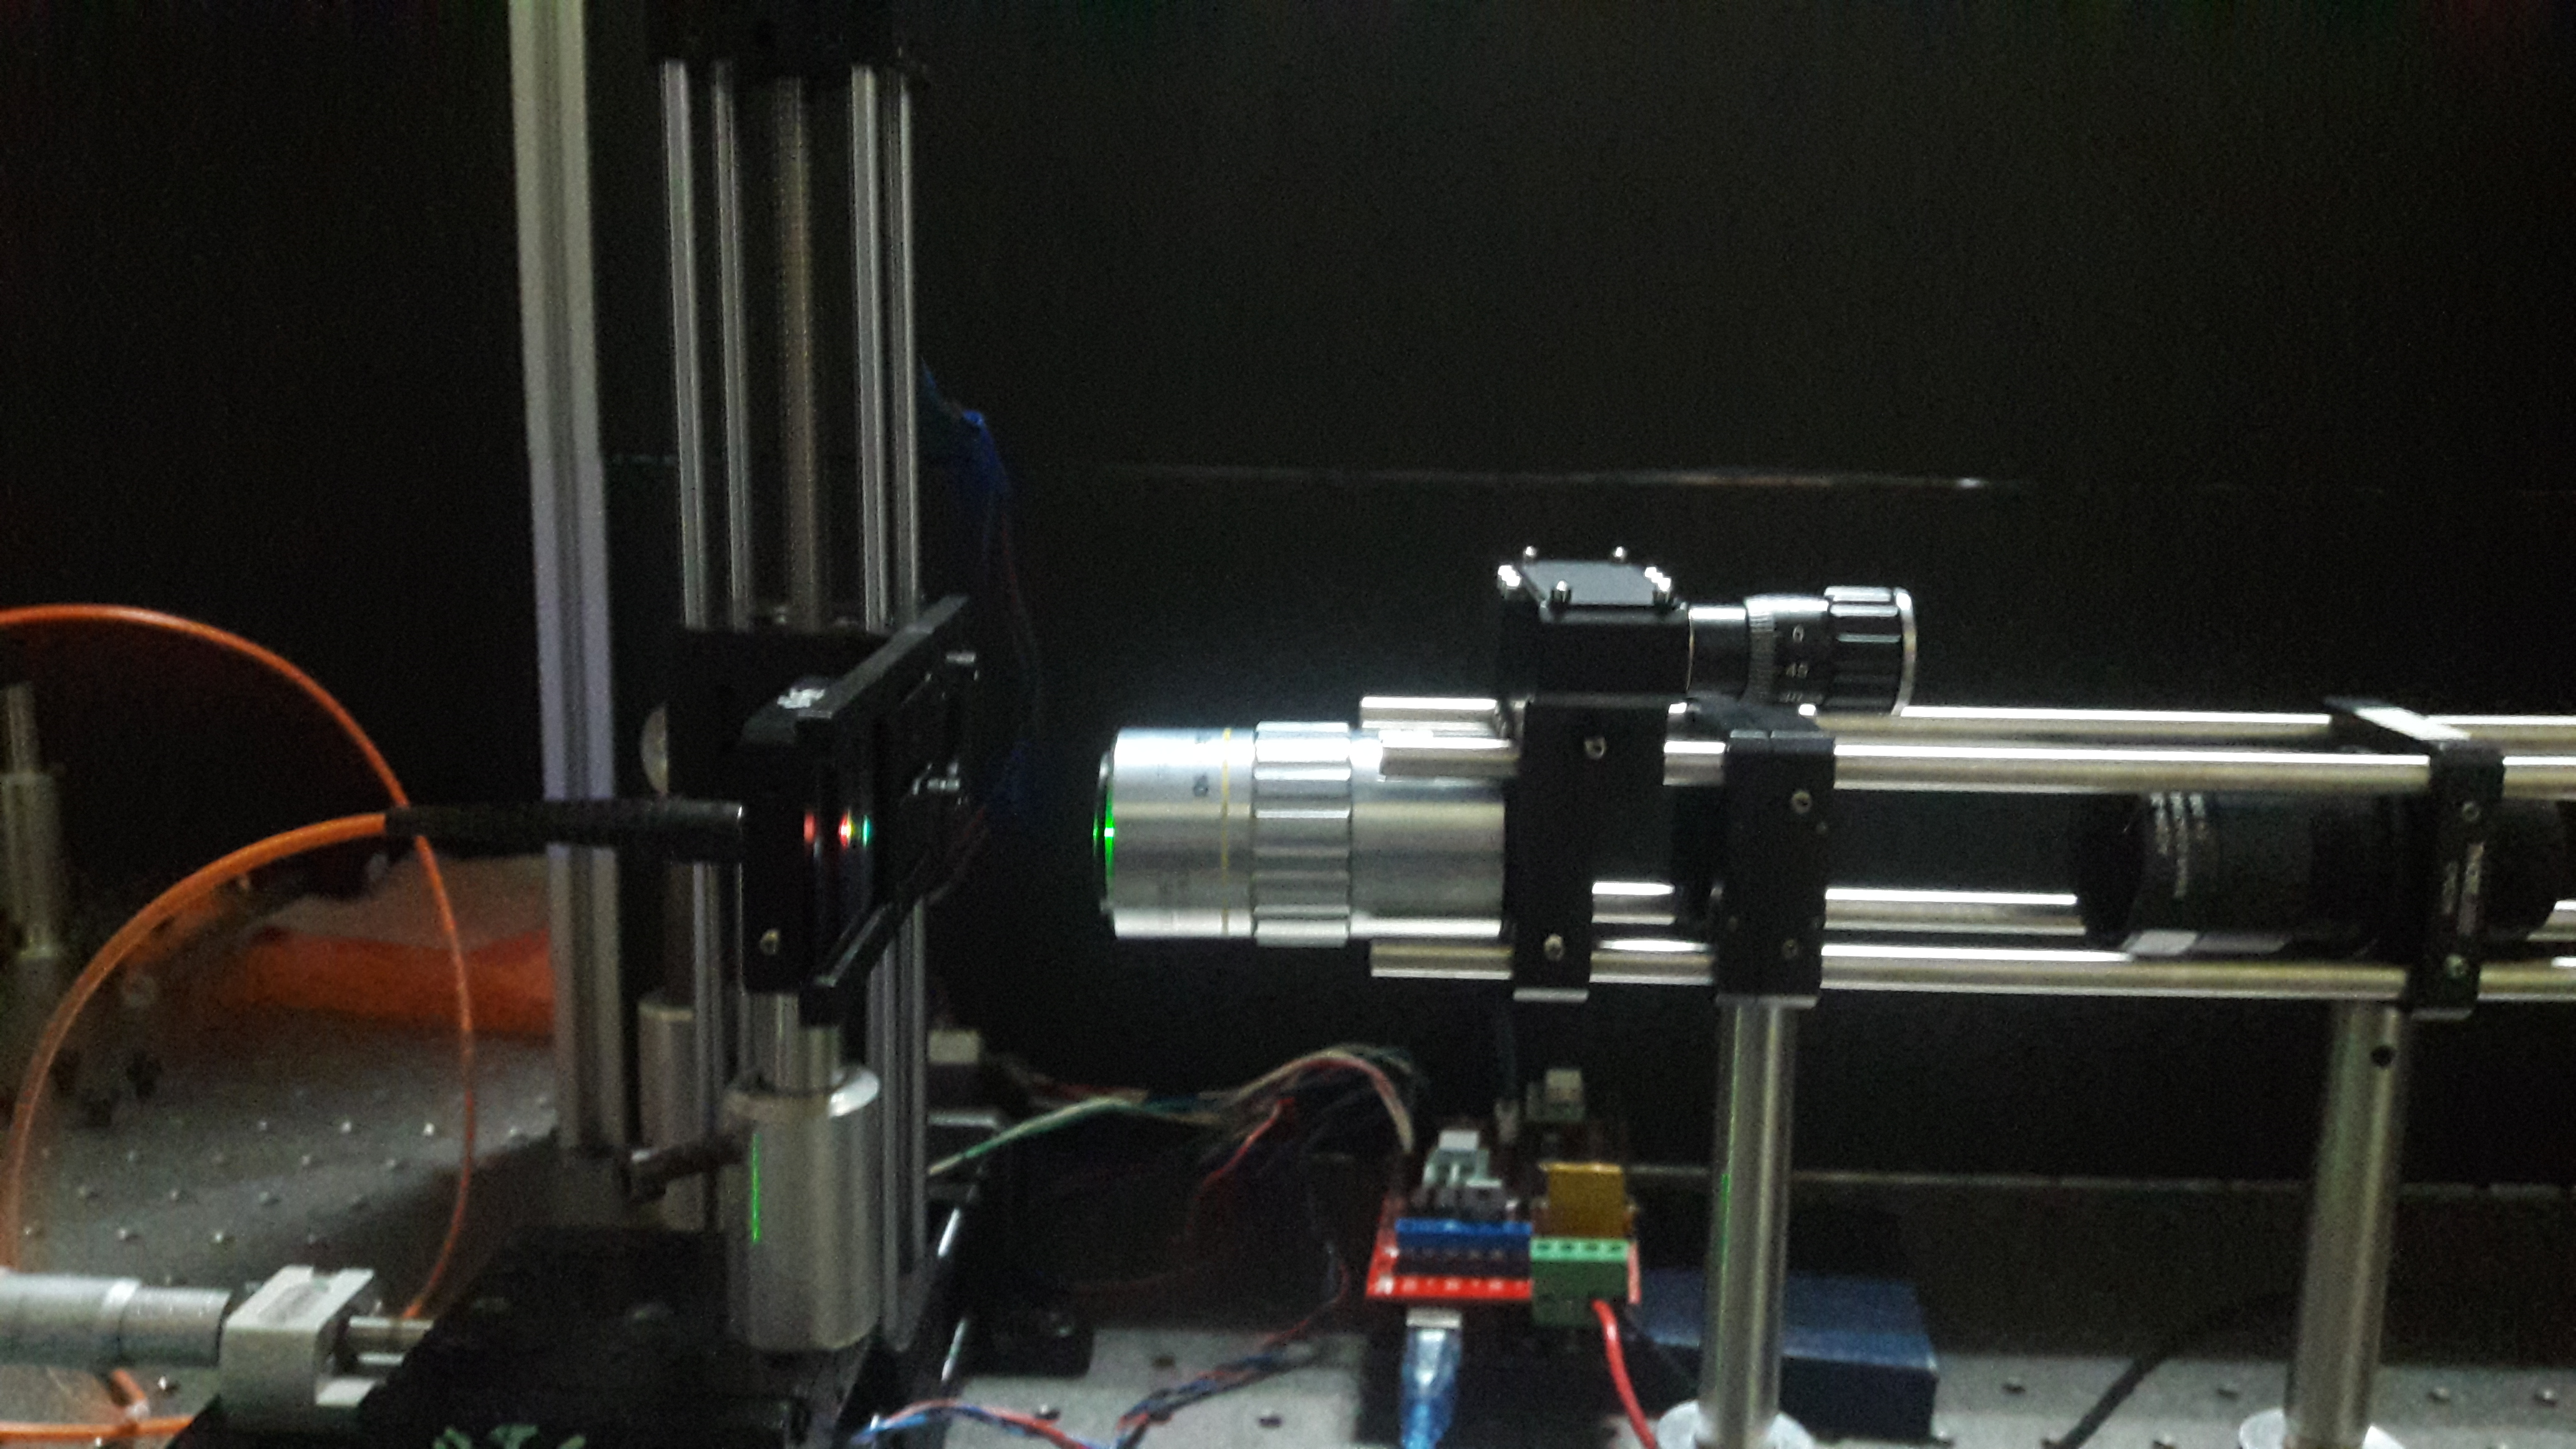
\includegraphics[scale=0.1]{Figs/microespectrometro/sm1zcambio.jpg}
	\caption{Visualización en la cámara de la reflexión del filtro de la iluminación.}
	\label{fig:bgcel}
\end{figure}


La idea es poner en foco el espectrómetro en alguna región del filtro, enfocar luego la cámara y después al mover el filtro a alguna otra región, tan solo hay que poner en foco el 'sistema' mirando la cámara. Al mismo tiempo si se quiere se puede volver a repetir el procedimiento de buscar el mínimo.


Gráfico de poner en foco el microespectrómetro: (19 de marzo)

mediciones guardadas en: data mediciones, simultaneidad, foco.

vamos recorriendo horario en pasos de 50 micrones en el SM1Z.
mediciones que consisten en un barrido de 80 micrones de largo, con pasos de 1 micron.. esto en la stage


RESULTADOS:

Z                  RESOLUCIÓN

0                  12.46 dudoso?

-50               13.5

-100             13.12

-150              12.87

-200              11.29

\singlespacing
\subsection{\textit{Software} automatizado de adquisición}
\label{sec:softadq}
\spacing{1.5}


\singlespacing
\subsection{Integración de una cámara web: adquisición simultánea de imágenes y de espectros de transmisión}
\label{sec:camwebgui}
\spacing{1.5}



\singlespacing
\section{Resultados}
\label{sec:resgrales}
\spacing{1.5}

\singlespacing
\subsection{Espectro de transmisión de cada banda del filtro}
\label{sec:espectransm}
\spacing{1.5}


\singlespacing
\subsection{Caracterización espectral de las manchas ó defectos de transmisión}
\label{sec:defctma}
\spacing{1.5}


\singlespacing
\subsection{Caracterización espectral de los agujeros ó huecos}
\label{sec:defctag}
\spacing{1.5}
